% !Mode:: "TeX:UTF-8"

\BiChapter{模型介绍}{}
在此考虑基于离散时间马氏链$\xi = (\xi_n)_{n \ge 0}$建模的随机热力学系统,该模型的状态空间是$S = \{1, \dots N\}$转移概率矩阵是$P=(p_{ij})_{i,j \in S}$,其中$p_{ij}$表示从状态$i$到状态$j$的转移概率。该马氏链对应的转移图为$G=(S, E)$,其中顶点集合$S$是状态空间,$E$是转移概率有向边的集合 \ref{figure:transitiongraph}。本文用$\langle i, j\rangle$表示状态$i$到状态$j$的有向边,因此有$E = \{\langle \langle i, j\rangle \in S \times S: p_{ij}>0\}$,并且令$|E| = M$,其中$|E|$表示集合$E$中元素的数量。本文所考虑的马氏链都是不可约的,也就是有向图$G$是连通的。因此对某个状态,图$G$不仅包含其他状态到其的边,还包括它到其自身的边,也就是自循环 \ref{figure:transitiongraph}。

转移图$G$中如果有一个如图 \ref{figure:transitiongraph}所示的图拓扑(除了自循环),将被视为一种特殊情形,在以往的研究中称该系统为单环马氏链。具体来说,如果马氏链$\xi$满足 $p_{ij}=0$且$|i-j| \ge 2$(其中的$i,j$是模$N$运算后的结果),则称为单环马氏链。单环系统在生物学方面具有特殊的意义。许多重要的生化过程,如酶和离子通道的构象变化\cite{cornish2013fundamentals,sakmann2013single},磷酸化-磷酸化循环\cite{beard2008chemical},甲基化-去甲基化循环\cite{jia2017nonequilibrium},以及染色体重塑导致的启动子的激活\cite{pedraza2008effects,jia2022analytical}都可以被建模为单环马氏链。下文中,主要关注单环系统,大部分的结论也可以扩展到一般系统。

\begin{figure}[h]\label{figure:transitiongraph}
\centering
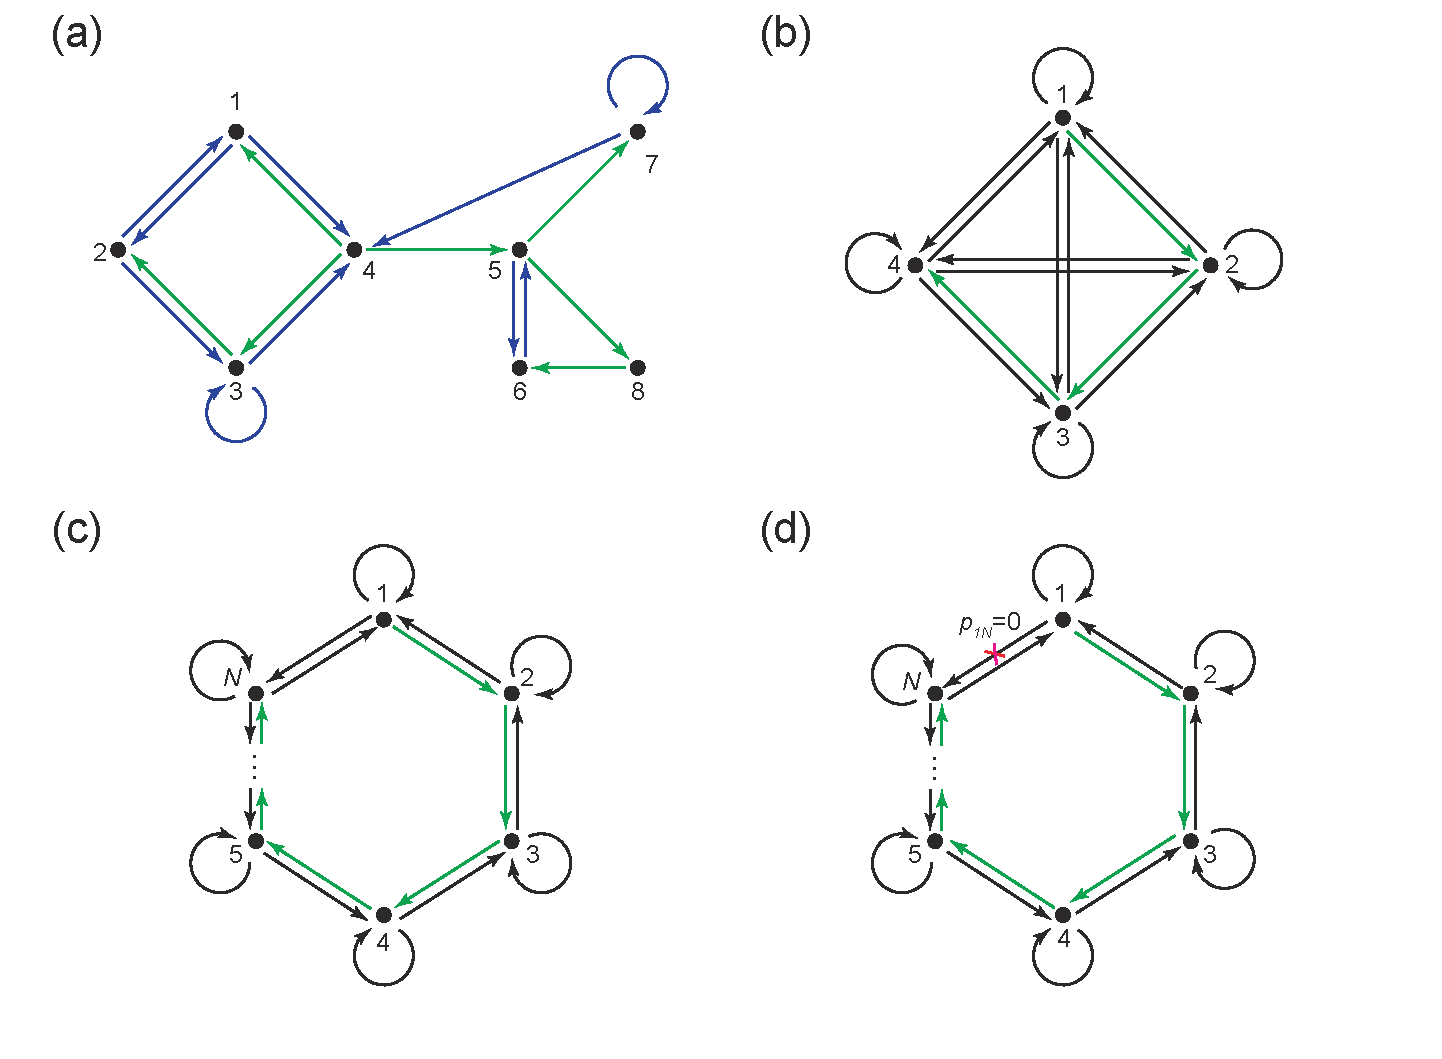
\includegraphics[scale=0.5]{chart/transitiongraph.pdf}
\caption{各类马氏链的转移图和相应的生成树 (a) 一般转移图的马氏链, 绿色线表示根节点为4的生成树$T$,并且蓝色线表示$T$的弦 (b) 四状态全连接马氏链,其中每个状态可以转移到自身和其他状态 (c) 
$N$状态单环马氏链。系统有一个环拓扑。每个状态转移到自身和它两个相邻节点 (d) 一个N状态的单环马尔科夫链,该系统无法从状态$1$转移到状态$N$ (b)-(d)中,绿色箭头表示生成树T}
\end{figure}

\BiSection{环擦除模式定义的环流}{}
本文调查和比较了马氏链中两种类型的环流。首先回顾环擦除模式定义的环流\cite{jiang2004mathematical,kalpazidou2007cycle}。马氏链中的回路是一个状态到自身的路径,比如路径$i_1 \to i_2 \to\cdots\to i_s \to i_1$(其中$i_1, i_2 , \cdots, i_s$是顶点集合$S$中不同点),其中$p_{i_1i_2}p_{i_2i_3}\cdots p_{i_si_1}>0$。令$j_1 \to j_2 \to\cdots\to j_r \to j_1$为另一个回路,若上述两个环满足存在一个整数$k$使得
\begin{equation*}
    j_1 = i_{k+1},j_2 = i_{k+2},\cdots,j_n = i_{k+s},
\end{equation*}
且$r=s$则称两个回路是等价的,其中指标$k+1,k+2,\cdots,k+s$被视为模$n$同余的。回路$i_1 \to i_2 \to\cdots\to i_s \to i_1$在上述等价关系下所属的等价类被表示为环$c = (i_1,i_2,\cdots,i_s)$。例如,$(1,2,3)$,$(2,3,1)$和$(3,1,2)$表示相同的环。定义环$(i_1,i_2,\cdots,i_s)$的反环为$(i_1,i_s,\cdots,i_2)$。系统中所用环的集合称为环空间$\mathcal{C}$。

沿着马氏链轨道的会不断形成各种类型的环。如果持续去除马氏链$\xi$中的环,并且在该过程中,持续聚焦在轨道中剩余状态的轨迹,那么将会获得一个新的马氏链$\tilde{\xi} = (\tilde{\xi}_n)_{n\geq 0}$,称其为导出链。例如,如果原始的马氏链$\xi$的轨道为$\{1,2,3,3,2,3,4,1,4,\cdots\}$,那么相应的导出链$\tilde{\xi}$的轨迹和形成的环为表 \ref{trajectory}所示。
\begin{table}[htb!]
    \renewcommand\arraystretch{1}\centering
    \begin{tabular}{cccccccccc} \hline\hline
   $n$            & 0 & 1 & 2 & 3   & 4     & 5 & 6 & 7         & 8 \\ \hline
   $\xi_n$         & 1 & 2 & 3 & 3   & 2     & 3 & 4 & 1         & 4 \\ \hline
   $\tilde{\xi}_n$& {[}1{]} & {[}1,2{]} & {[}1,2,3{]} & {[}1,2,3{]} & {[}1,2{]} & {[}1,2,3{]} & {[}1,2,3,4{]} & {[}1{]} & {[}1,4{]} \\ \hline
    \text{形成的环} &   &   &   & (3) & (2,3) &   &   & (1,2,3,4) &   \\ \hline\hline
    \end{tabular}
    \caption{导出链和形成环的案例}\label{trajectory}
\end{table}

确切地说,导出链的状态是$S$的中不同状态组成的有限序列,表示为$[i_1,i_2,\cdots,i_s]$。假设$\tilde{\xi}_{n-1}=[i_1,i_2,\cdots,i_s]$且$\xi_n = i_{s+1}$。若$i_{s+1}$不同于$i_1,i_2,\cdots,i_s$中任意一个,那么$\tilde{\xi}_n$被定义为$\tilde{\xi}_n = [i_1,i_2,\cdots,i_s,i_{s+1}]$。其次,若$i_{n+1}=i_r, \forall 1 \le r\le s$,那么$\tilde{\xi}_n$被定义为$\tilde{\xi}_n = [i_1,i_2,\cdots,i_r]$。对于这种情况,称马氏链在时间$n$形成环$(i_r,i_{r+1},\cdots,i_s)$。令$N^c_n$为环$c$在时间$n$时形成的次数。那么在时间$n$时,环$c$的经验环流可以被定义为:
\begin{equation*}
    J_n^c = \frac{1}{n}N^c_n,
\end{equation*}
并且在时间$n$时,经验净环流可以定义为:
\begin{equation*}
    \tilde{J}^c_n = J^c_n-J^{c-}_n.
\end{equation*}
用更直观的表述,$J^c_n$表示环$c$每个单位时间形成的数量,$\tilde{J}^c$表示环$c$每个单位时间形成的净数量。多数研究只多关注净环流的性质 \cite{Schnakenberg1976NetworkTO,andrieux2007fluctuation,andrieux2007network},本文还会关注环流的性质。
若令$n\rightarrow\infty$,则有经验环流$J^c_n$和 经验净环流$\tilde{J}^c$分别以概率为 1 趋近于$J^c$和$\tilde{J}^c$。
极限$J^c$和$\tilde{J}^c$分别为环$c$的环流和净环流。关于$J^c_n$和$\tilde{J}^c$更为细致的描述,可以参考文献 \cite{jiang2004mathematical}。著名的环流分解定理 \cite{jiang2004mathematical} 可以用上述定义写为:
\begin{equation}\label{decomposition}
    \pi_ip_{ij} = \sum_{c\ni\langle i,j\rangle}J^c,
\end{equation}
其中求和项考虑到了所有通过边 $\langle i, j\rangle$ 的环 $c$(符号 $c \ni \langle i, j\rangle$表示环$c$通过边$\langle i, j\rangle$)。这表明任意状态对的概率流可以分解为环流的和。

\BiSection{生成树定义的环流}
环流也可以通过生成树定义 \cite{Schnakenberg1976NetworkTO,kalpazidou2007cycle}。令$T$为转移图$G$的有向子图,即$T$的所有边也是$G$的边,且令$\hat{T}$表示$\bar{T}$表示与$T$有关的无向图。满足下列三个条件的$T$被称为图$G$的生成树(极大树):
\begin{itemize}
    \item $T$是$G$的覆盖子图,即$T$包含$G$的所有顶点。
    \item $\bar{T}$是连通的。
    \item $\bar{T}$没有回路,其中无向图的回路是顶点到自身的无向路径。
\end{itemize}

下文使用$T$来表示生成树本身和它的边集合。一般情况,生成树的选择不是唯一的,一个图可能有许多不同的生成树。易知任何生成树$T$必须包含$G$的的所有顶点,并且必须有$N-1$条边(见图 \ref{figure:transitiongraph}中的绿色箭头)\cite{kalpazidou2007cycle}。

% 易知生成树$T$包含$G$的所有顶点,并且$|T| = N -1$。接下来,会通过$T$表示生成树和它的边集合。图的生成树并不唯一,一个图可以有很多完全不同的生成树。

有向边$l \notin T$被称为$T$的弦(见图 \ref{figure:transitiongraph}(a)中的蓝色箭头)。因为$|E|=M$且$|T|= N-1$,所以任意生成树$T$都有$M-N+1$个弦。由于$\bar{T}$是连通的且没有回路,如果添加一根弦$l$到$T$,将会导致无向子图$\overline{T \cup \{l\}}$必有恰好一个回路。记$c_l$是从这个回路中获得的环,并且和$l$保持同样的指向。例如图 \ref{figure:transitiongraph}(c) 中所示的系统,如果在生成树$T$中添加弦 $l=\langle 2,1 \rangle$(蓝色箭头所示),那么可以得到环 $c_l=(2,1,4,3)$。由由弦生成的环的集合$\mathcal{L} = \{c_l: l\in E\setminus T\}$被称为基本集。
由于弦和基本集之间一一对应的关系,可以用$c_l$形成的次数定义通过弦$l$的次数。在$n$时刻,$c_l$的经验环流可以被定义为:
\begin{equation*}
    Q^{c_l}_n = \frac{1}{n}\sum_{i=1}^n1_{\{\langle\xi_{i-1},\xi_i\rangle=l\}}.
\end{equation*}
$Q^{c_l}_n$表示单位时间通过弦$l$的次数。生成树方式和环擦除方式有很大的不同,环擦除可以很便捷的定义环流,生成树只能定义基本集的环流。

%%%%%%%%%%%%%%%%%%%%%%%%%%%%%%%%%%%%%%%%%%%%%%%%%


类似的,也可以用生成树方式定义净环流。最终,假设转移概率满足$p_{ij}>0$,当且仅当$p_{ji}>0$;这个条件可以保证系统的熵增量是有限值\cite{Schnakenberg1976NetworkTO,jiang2004mathematical}。对于任意弦$l$,在时间步$n$,$c_l$的净环流定义为:
\begin{equation*}
    \tilde{Q}^{c_l}_n=Q^{c_l}_n-Q^{c_l-}_n.
\end{equation*}
如果$c_l$中只有一个或两个状态,那么$c_l = c_{l^-}$,因此$\tilde{Q}_n^{c_l}=0$。对于弦$l=\langle i,j \rangle$,如果$c_l$中有三个及以上的状态,那么$l^-=\langle j,i\rangle$也是一个弦,并且$c_{l^-}$恰好是由弦$l^-$生成的环。在文献 \cite{Schnakenberg1976NetworkTO, andrieux2007fluctuation, andrieux2007network},净环流的只针对有三个及以上状态的的环定义,本文参考\cite{kalpazidou2007cycle}中的定义,使得净环流的定义也可以包含只有一个或两个状态的环。

若$n \to \infty$, 则经验环流$Q_n^{c_l}$和经验净环流$\tilde{Q}_n^{c_l}$将会分别以概率为$1$趋于$Q^{c_l}$和$\tilde{Q}^{c_l}$。极限$Q^{c_l}$和$\tilde{Q}^{c_l}$分别作为环$c$的环流与净环流。对于弦$l=\langle i,j \rangle$,依据马氏链的遍历性,有$Q^{c_l} = \pi_i p_{ij}$。

\BiSection{两种类型环流的比较}{}
下面将简述两种类型环流的差异。为讨论过程更加清晰,下面称环擦除方式定义的环流称为$LE$环流,生成树方式定义的环流称为$ST$环流。$LE$环流是定义在整个环空间$\mathcal{C}$,然而$ST$环流仅是针对基本集$\mathcal{L}$中的环定义。因此,从环动力学角度,$LE$环流相较于$ST$环流给出了更完整的描述。而且,由于生成树一般并不唯一,不同的生成树选择会对应不同的$ST$环流。相比之下,$LE$环流并不依赖生成树的选择。

经过论述,自然会问到基本集$\mathcal{L}$相比环空间$\mathcal{C}$小多少。因为每根弦对应集合$\mathcal{L}$唯一一个元素,有$|\mathcal{L}| = |E\setminus T| = M-N+1$,所以很难对$|\mathcal{C}|$给出统一的表达。为了得到更深刻的观点,下面关注两个特殊的案例。首先考虑转移图是全连接的马氏链,即$p_{ij}>0, \forall i,j \in S$,如图 \ref{figure:transitiongraph}(b)。其中包含$k$个状态的环的数量是$\frac{N (N-1) \cdots (N-K+2)(N-k+1)}{k}$,因此
\begin{equation*}
    |\mathcal{C}| = \sum_{k=1}^N\frac{N\cdots (N-k+1)}{k}.
\end{equation*}
特别的,当$N=4$,有$|\mathcal{C}|=24$,环空间为:
\begin{align*}
    \mathcal{C} = \{&(1),(2),(3),(4),(1,2),(1,3),(1,4),(2,3),(2,4),(3,4),\\
    &(1,2,3),(1,2,4),(1,3,2),(1,3,4),(1,4,2),(1,4,3),(2,3,4),(2,4,3),\\
    &(1,2,3,4),(1,2,4,3),(1,3,2,4),(1,3,4,2),(1,4,2,3),(1,4,3,2)\}.
\end{align*}
若选定生成树$T = 1\to 2\to 3\to 4$,那么有$|\mathcal{L}|=13$,基本集为:
\begin{align*}
    \mathcal{L} = \{&(1),(2),(3),(4),(1,2),(2,3),(3,4)\\
    &(1,2,3),(1,3,2),(2,3,4),(2,4,3),(1,2,3,4),(1,4,3,2)\}.
\end{align*}
因此对于全连接系统,$ST$环流会比$LE$环流小很多。

接下来考虑单环马氏链 \ref{figure:transitiongraph}(c)。为了叙述方便,假设任意一对相邻状态$i$和$j$满足$p_{ii}>0$和$p_{ij}>0$。这里,$|\mathcal{C}| = 2N +2$,并且环空间为:
\begin{equation}\label{cycle_space}
    \mathcal{C} = \{(1),\cdots,(N),(1,2),\cdots,(N-1,N),(N,1),(1,2,\cdots,N),(1,N,\cdots,2)\}.
\end{equation}

其中前$N$个环是只包含一个状态的环,即自循环的。中间$N$个环是两状态的环,最后两个环是$N$个状态的环。如果选定生成树$T = 1\to 2\to\cdots \to N$,那么有$|\mathcal{L}| = 2N + 1$,并且基本集是:
\begin{equation*}
    \mathcal{L} = \{(1),\cdots,(N),(1,2),\cdots,(N-1,N),(1,2,\cdots,N),(1,N,\cdots,2)\}.
\end{equation*}
对于单环系统,只有环$(N, 1)$在环空间$C$中,却没有在基本集$\mathcal{L}$中。

为了进一步理解经验$LE$环流$J_n^c$和经验$ST$环流$Q_n^{c_N}$的关系,面使用周期边界条件假设,即$\xi_0 = \xi_1$,这也是文献\cite{den2000large}中标准的假设条件。基于这个假设,对任意弦$l$,易得:
\begin{equation}\label{conversion}
    Q_n^{c_l} = \sum_{c\in\mathcal{C}}J^c_n1_{\{l\in c\}}.
\end{equation}
其中求和项考虑到了所有通过弦$l$的环 $c$(符号$c \ni l$表明$c$通过状态$i$)。注意到上述方程两边都表示弦$l$单位时间按形成的数量。这说明经验$ST$环流可以表示为经验$LE$环流的线性组合。
